	\begin{figure}[!bhp]
	\centering
		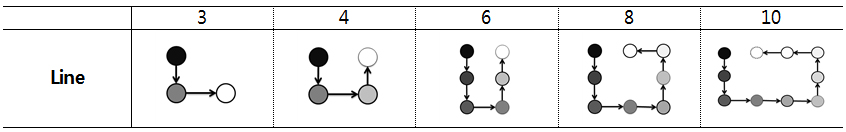
\includegraphics[height=50pt]{Topologies_Line}
		\caption{Bayesian Network Topology : Line}
	\end{figure}	

	% Line 형태는 자식 node의 자식 node, 또 그 자식 node가 계속 이어지는 형태를 말한다. 마치 그 모습이 line과 같다.
	Line forms, child node of the child node, also refers to the form in which the child node is followed by continuation. Though the figure is as of line.

	\begin{figure}[!bhp]
	\centering
		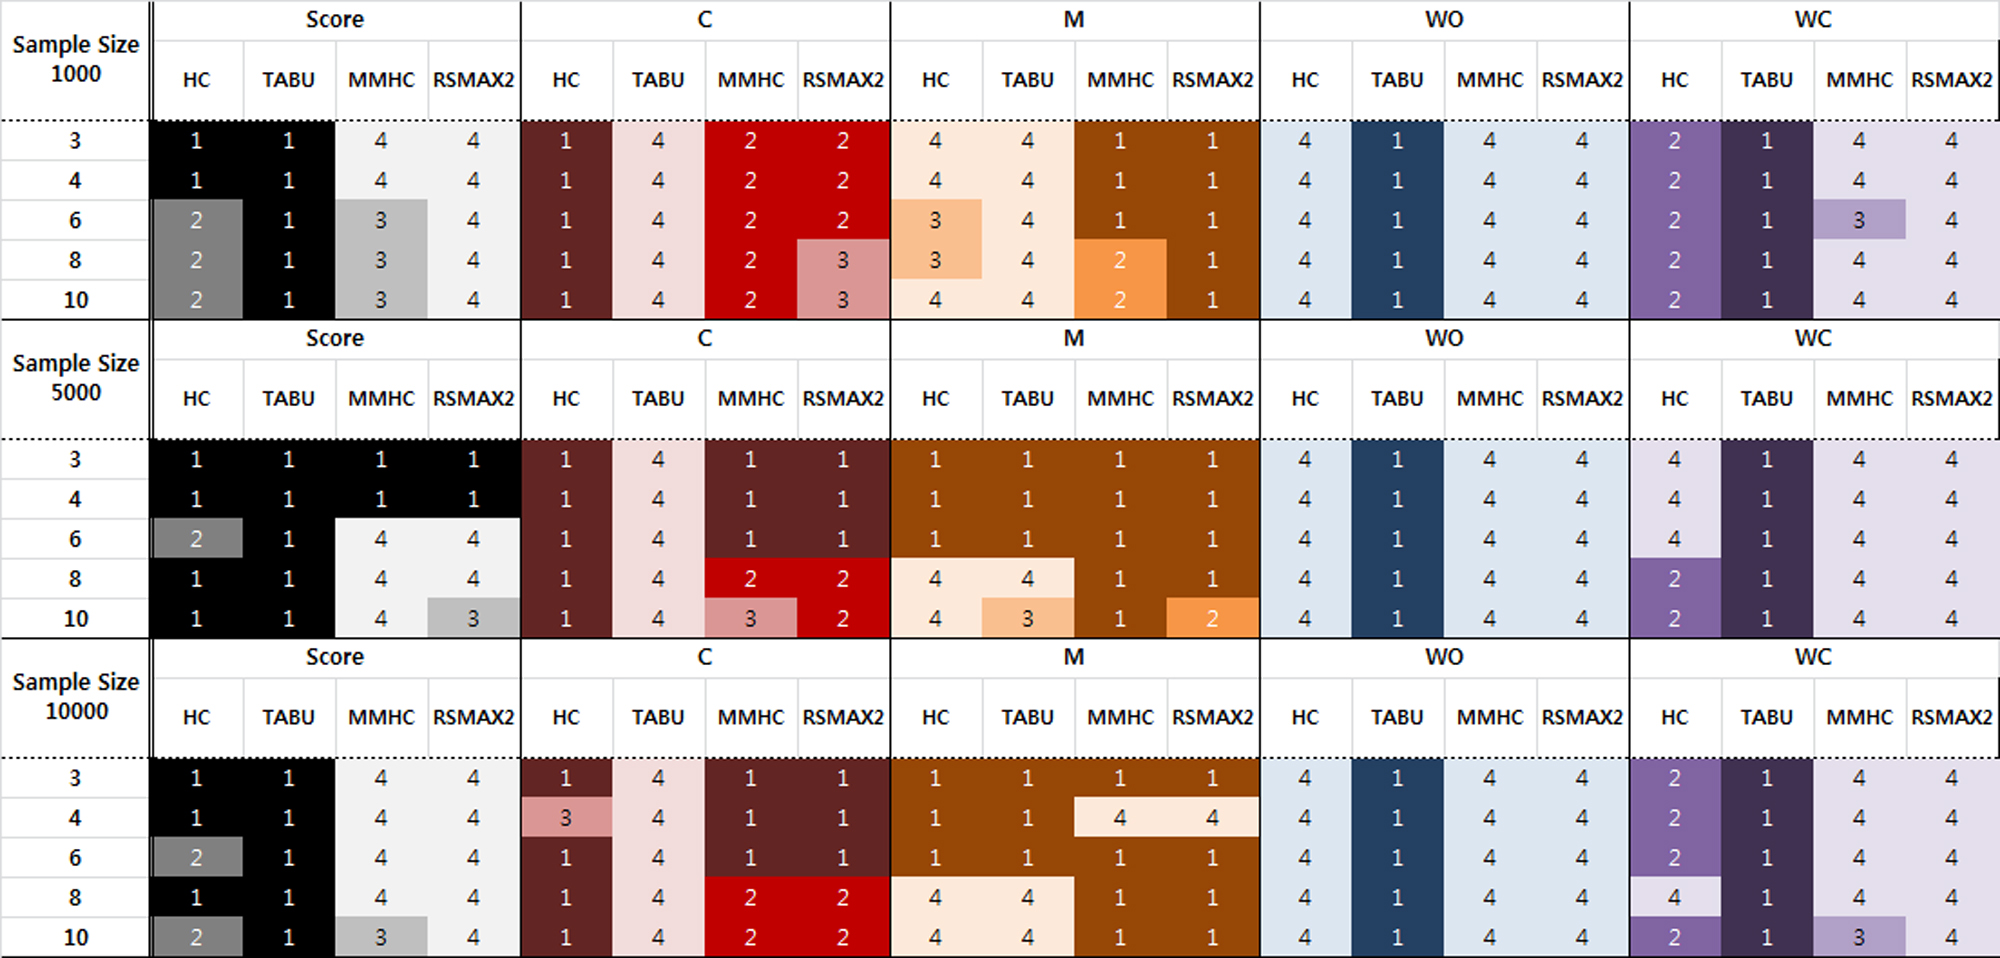
\includegraphics[height=170pt]{Result_Line}
		\caption{Summary for Comparison via Line}
	\end{figure}	
	
% 다른 topology에 비해 알고리즘별 성능이 크게 차이가 발생하지 않았다.
Performance of each algorithm is compared to other topology were not different significantly occurs.

% 그러나 TABU search는 score에 따른 성능이 좋음에도 불구, 다른 알고리즘에 비해 C의 개수가 압도적으로 적고, M, WO, WC의 개수가 무척 높은 모습이 나타났다.
However, TABU search, despite good performance by score, the number of C is overwhelmingly smaller than the other algorithms, M, WO, very high figure is the number of WC revealed.

% 상대적으로 Hill-climbing이 line 형태에 대해 좋은 성능을 보여주었다.
Relatively Hill-climbing has showed good performance for line form.

	\begin{figure}[p]
	\centering
		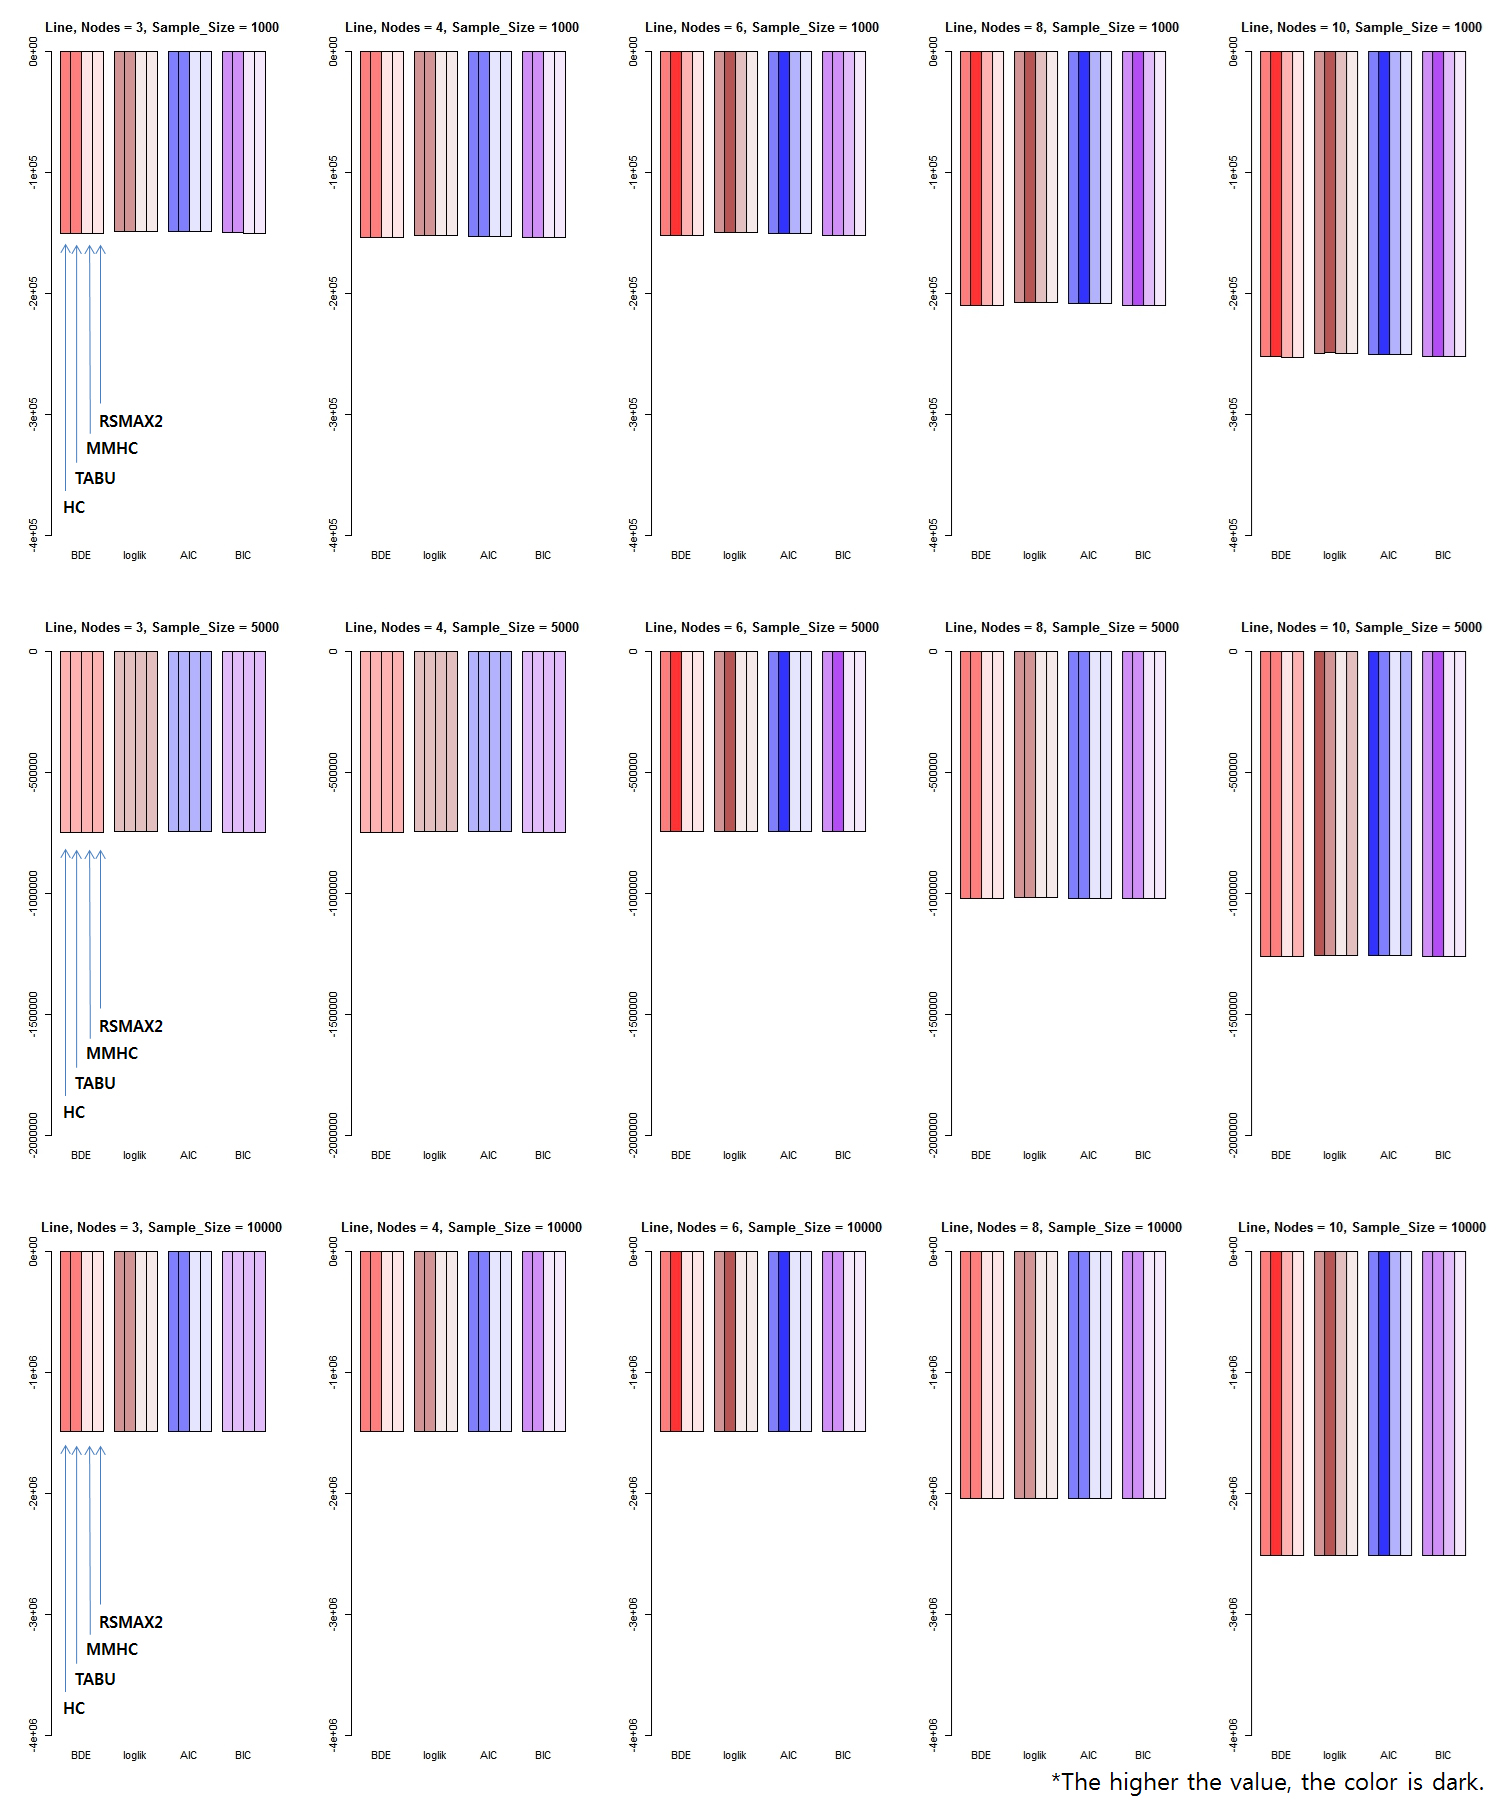
\includegraphics[height=500pt]{02_Line_Score}
		\caption{Comparison of scores via Line}
	\end{figure}	

	\begin{figure}[p]
	\centering
		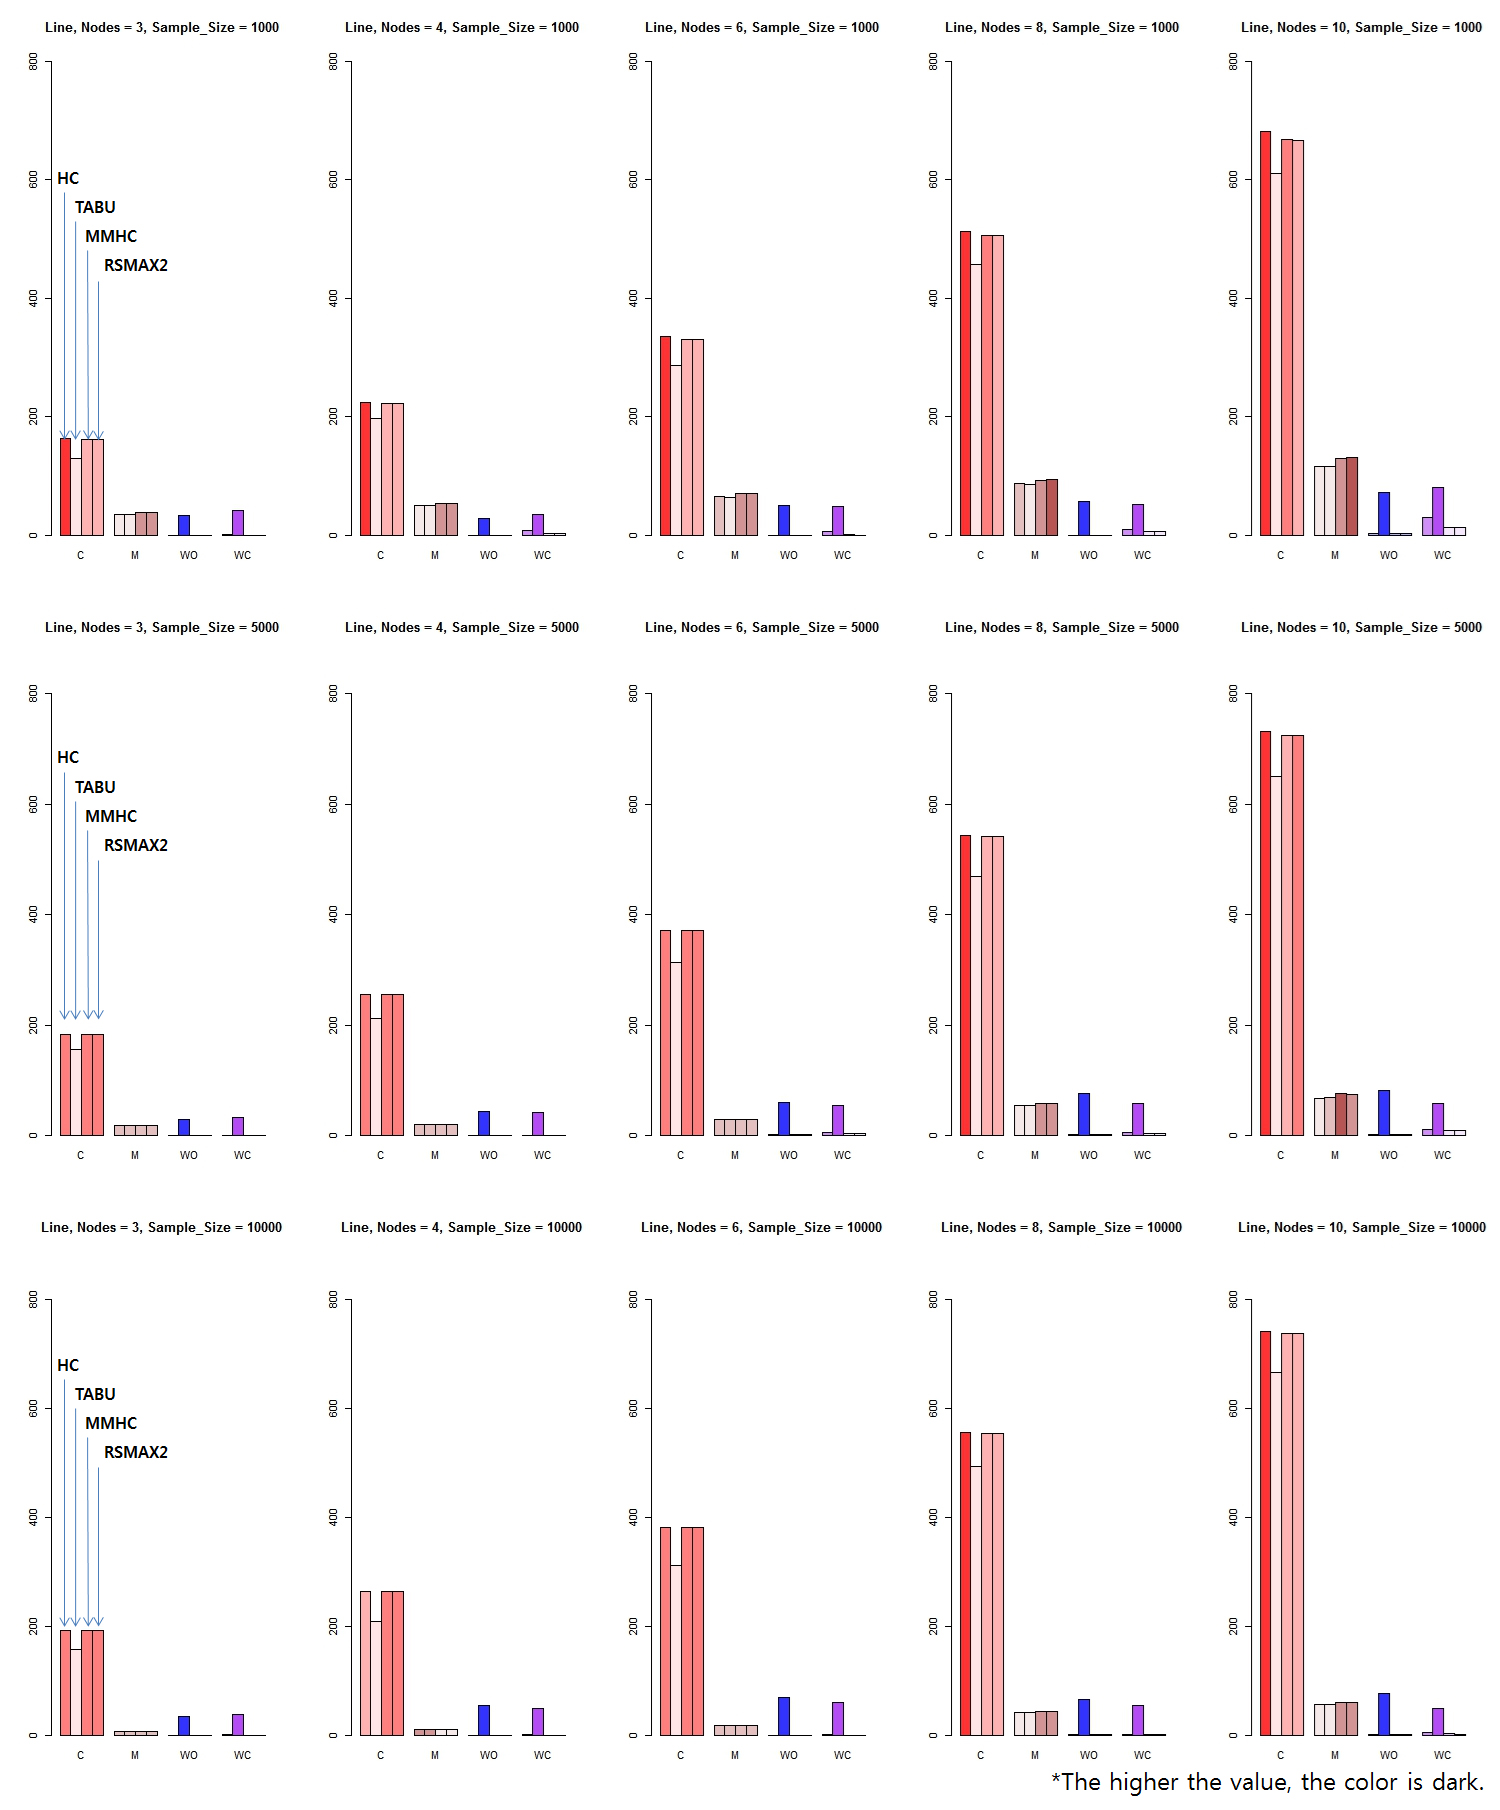
\includegraphics[height=500pt]{02_Line_Arcs}
		\caption{Comparison of correct arcs via Line}
	\end{figure}	
